\section{Resultados}
En esta sección incluiremos los resultados de la experimentación que realizamos con el perceptrón desarrollado.\\
La idea general de los experimentos es intentar medir la influencia de alguna(s) variable(s) específicas sobre la performance
de la red. Para ello intentamos fijar todas las demás variables en valores óptimos y poner a prueba las que nos interesaban.\\

A medida que fuimos encontrando valores óptimos para las distintas variables, los fuimos utilizando para el resto de los experimentos subsiguientes.\\

En el primer experimento, intentamos determinar el mejor número de capas ocultas para utilizar en el ejercicio 1. A continuación, los resultados.

\subsection{Ejercicio 1}

\subsubsection{Variación del número de capas ocultas.}
La idea de este experimento es determinar la cantidad de capas ocultas óptimas para el ejercicio 1. Para ello fijamos las demás variables con esta configuración:

\begin{itemize}
\item Épocas: 250
\item ETA: 0.05
\item 10 neuronas por capa.
\item 70 \% del dataset como training, 20 \% training, 10\% validación.
\item Distribución de Pesos: Normal
\item Batch Estocástico
\item Sin Momentum
\item Sin Early Stopping
\end{itemize}

Esta configuración es arbitraria y está basada en pruebas informales que realizó el equipo antes de comenzar la experimentación formal. A medida que avanzaron los experimentos y fuimos descubriendo mejores valores, los fuimos actualizando para las siguientes pruebas.\\

El experimento fue desarrollado así: 
\begin{itemize}
\item Dividimos el dataset en datos de entrenamiento, validación y testing. Utilizamos la misma división para todas las ejecuciones.
\item Con la configuración mencionada, corrimos 8 rondas de cada número de capas ocultas utilizando: 1, 2, 3, 5 y 10 capas.
Es decir, primero se ejecutaron 8 veces el entrenamiento, validación y testing de una red con 1 capa. Luego repetimos con 2, con 3, etc.
\item Para cada cantidad de capas, promediamos los resultados de cada una de las 8 rondas. Con ello obtuvimos un error final (función de costo) de entrenamiento promedio , un error de validación promedio y una efectividad de testing promedio. Llamamos efectividad de testing a la cantidad de resultados del dataset de testing correctamente predichos.
\item El error final de cada ronda corresponde a la función de costo de dicha corrida dividido la cantidad de patrones procesados.
\end{itemize}

Observemos los resultados:\\

\begin{figure}[h]
  \begin{center}
  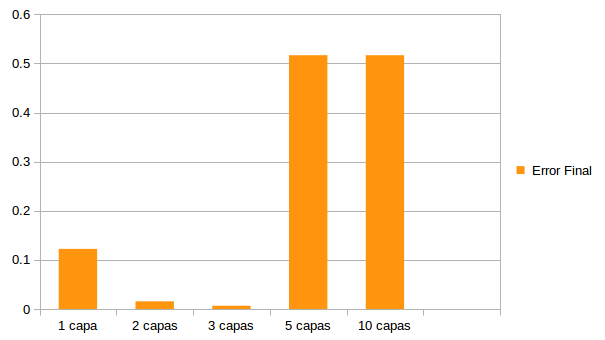
\includegraphics[scale=0.75]{graficos/fig1_cant_capas_error_final.png}
  \caption{Error final (función de costo) promedio para cada cantidad de neuronas utilizando el dataset de entrenamiento}
  \end{center}
\end{figure}

Podemos ver en la figura 1 que los mejores errores fueron obtenidos con 2 y 3 capas. Estos datos pertenecen al error final promediado, usando el dataset de entrenamiento.\\
Notamos también que con más de 3 capas ya los números se empiezan a distorsionar y perder mucha precisión.

Para el error final en los datos de validación, obtuvimos los siguientes resultados:\\

\begin{figure}[h]
  \begin{center}
  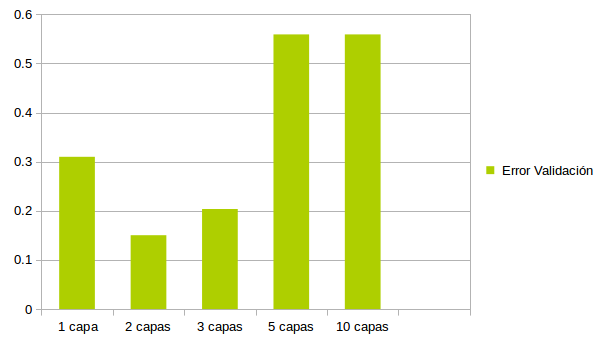
\includegraphics[scale=0.75]{graficos/fig2_cant_capas_error_valid.png}
  \caption{Error (función de costo) promedio para cada cantidad de neuronas utilizando el dataset de validación}
  \end{center}
\end{figure}


En la figura 5 podemos notar que el valor de error con el dataset de validación también 
genera mejores números con 2 y 3 capas. Especialmente se aprecia un mejor valor para la arquitectura de 2 capas.\\
Observamos nuevamente que los valores más altos no rinden igual de bien que los anteriores.

\begin{figure}[h]
  \begin{center}
  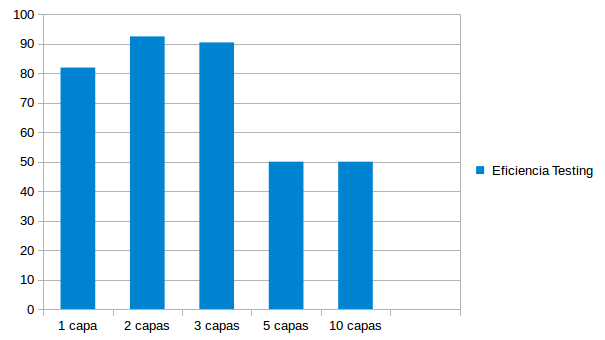
\includegraphics[scale=0.75]{graficos/fig3_cant_capas_testing.png}
  \caption{Tasa de predicciones correctas, en porcentaje, para el dataset de testing}
  \end{center}
\end{figure}

Para la efectividad en la predicción de los datos de testing, observamos que la red de 1 capa generó aciertos cercanos al 82\%, mientras que las de 2 y 3 capas superan el 90\%, teniendo la de 2 capas un desempeño levemente mejor.\\
Nos sorprendíó ver que las redes de 5 y 10 capas lograron una muy baja eficiencia, cercana al 50\%.\\

Teniendo en cuenta los resultados presentados en estas pruebas, nos decidimos por una arquitectura de 2 capas ocultas. Aunque se obtuvieron resultados casi igual de buenos con arquitectura de 3 capas, \textbf{la de 2 capas presenta mejor velocidad de ejecución y resultados levemente mejores}.\\

\newpage

\subsubsection{Variación del número de neuronas ocultas.}

Una vez obtenido el número óptimo de capas ocultas, quisimos determinar cual era la cantidad de nueronas que debía contener
cada una de estas capas. Para simplificar el problema, decidimos que todas las capas tuvieran la misma cantidad de neuronas.\\
De esta forma, elegimos las siguientes medidas: 2 capas de 2, 5, 7, 10, 15 y 20 neuronas. Estas medidas fueron elegidas para intentar representar una cantidad baja de neuronas como 2,5,7 y otras más altas, por arriba de 10. No consideramos cantidades mayores de neuronas ya que los resultados no mejoran ostensiblemente pasando las 20 neuronas, teniendo en cuenta la relativa
sencillez del ejercicio en cuestión. Además, arquitecturas con más de 20 neuronas por capa afectan notablemente la velocidad de ejecución de la red, relentizando las pruebas y haciéndolas engorrosas e innecesarias.\\

De forma similar al experimento anterior, esta prueba consistió en procesar el dataset completo 8 veces con cada cantidad de neuronas distintas, promediar los errores finales de entrenamiento y de validación junto con la eficiencia obtenida en los datos de testing.\\
Para el error final, obtuvimos los siguientes resultados:\\

\begin{figure}[h]
  \begin{center}
  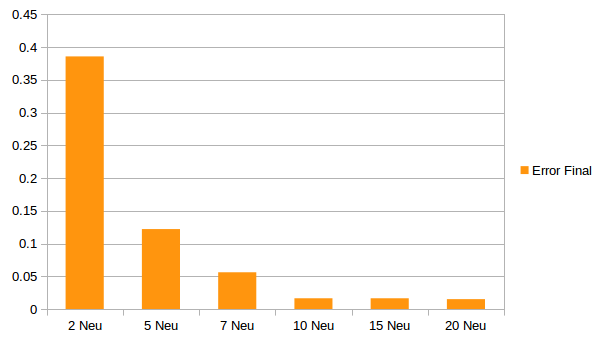
\includegraphics[scale=0.75]{graficos/fig4_cant_neuro_error_final.png}
  \caption{Error final (función de costo) promedio para cada cantidad de neuronas utilizando el dataset de entrenamiento}
  \end{center}
\end{figure}

En la figura 4 se puede observar que el valor de la función de costo decrece a medida que la cantidad
de neuronas crece. Este efecto se vuelve mucho menos notable a partir de las 10 neuronas por capa.\\

Para el error final en los datos de validación, obtuvimos los siguientes resultados:\\

\begin{figure}[h]
  \begin{center}
  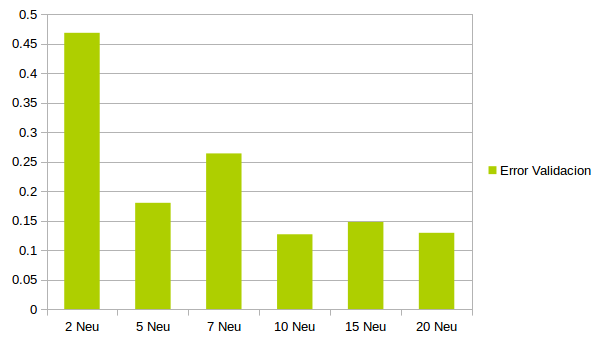
\includegraphics[scale=0.75]{graficos/fig5_cant_neuro_error_valid.png}
  \caption{Error (función de costo) promedio para cada cantidad de neuronas utilizando el dataset de validación}
  \end{center}
\end{figure}

En la figura 5 podemos notar que el valor de error con el dataset de validación también decrece a medida que sube la cantidad
de neuronas, aunque no de forma uniforme. Podemos apreciar que a partir de las 10 neuronas, el error se mantiene por debajo de 0.15.\\

Para la efectividad en la predicción de los datos de testing, observamos:\\

\begin{figure}[h]
  \begin{center}
  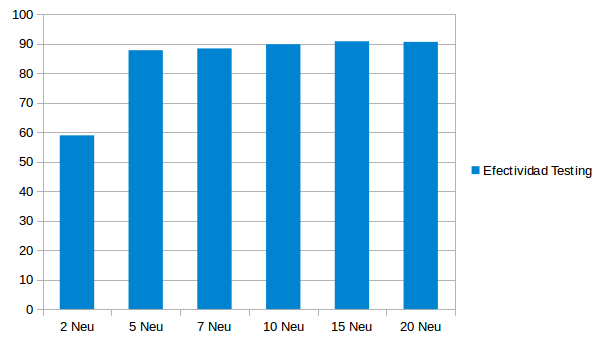
\includegraphics[scale=0.75]{graficos/fig6_cant_neuro_testing.png}
  \caption{Tasa de predicciones correctas, en porcentaje, para el dataset de testing}
  \end{center}
\end{figure}

Nuevamente podemos apreciar en la figura 6, que a medida que crece la cantidad de neuronas, crece la cantidad de aciertos sobre el conjunto de datos de test. Sin embargo, los resultados se comienzan a estancar a partir de las 10 neuronas en valores cercanos al 90 \% de aciertos.\\

Observando los resultados obtenidos en las pruebas, decidimos que la mejor configuración es con 10 neuronas por capa. Esta decisión se justifica teniendo en cuenta que los resultados no mejoran demasiado pasando de 10 y si empeora notablemente la velocidad de la red.\\
Por ende, \textbf{en vistas a los buenos resultados obtenidos con 10 neuronas y no obteniendo mejoras sustanciales con cantidades mayores}, nos quedaremos con este valor.

\subsubsection{Performance de la red, con entrenamiento sin momentum y con momentum.}

El momentum es una memoria o inercia que nos permite que los cambios en el vector de pesos $w$ sean suaves ya que incluyen información sobre el cambio de peso anterior. 
En el proceso de backpropagation de la red, cuando actualizamos los pesos, utilizaremos el momentum de la siguiente manera:
\\
\\
$\Delta w_{ij}^{m} = \eta \delta_{i}^{m}V_{j}^{m} + \alpha \Delta w_{pq}^{m-1}$
\\

Para este experimento, mantenemos la configuración que veniamos utilizando en experimentos anteriores con 2 capas de 10 neuronas. Probaremos el comportamiento de la red 
variando el momentum desde $0$ (o sin momentum) hasta un valor de momentum de $0.9$. No utilizaremos valores mayores de $0.9$ ya que significaría que el peso anterior que 
tenía el eje se estaría acumulando con el nuevo peso en su completitud, lo cual nos parece una exageración en este caso. Dado que en posteriores experimentos realizaremos
pruebas variando el momentum y el learning rate en conjunto, para este experimento, mantendremos el learning rate de $0.05$.

\begin{figure}[!htbp]
\centering
\begin{subfigure}{.5\textwidth}
  \centering
  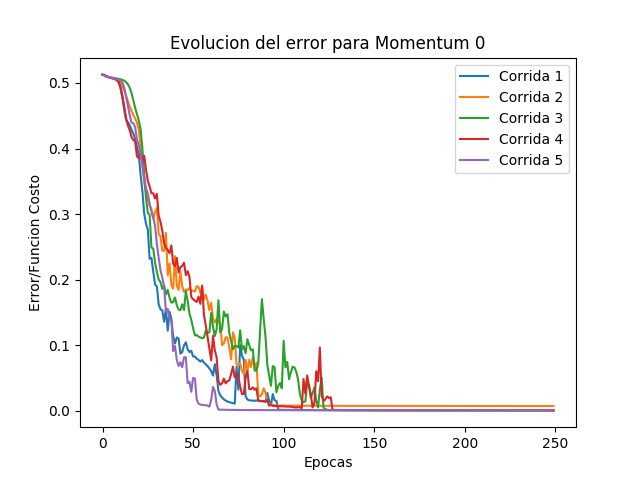
\includegraphics[width=1\linewidth]{graficos/momentum_0.png}
  \caption{Evolución del error de entrenamiento para momentum 0 (sin momentum)}
  \label{fig:sub1}
\end{subfigure}%
\begin{subfigure}{.5\textwidth}
  \centering
  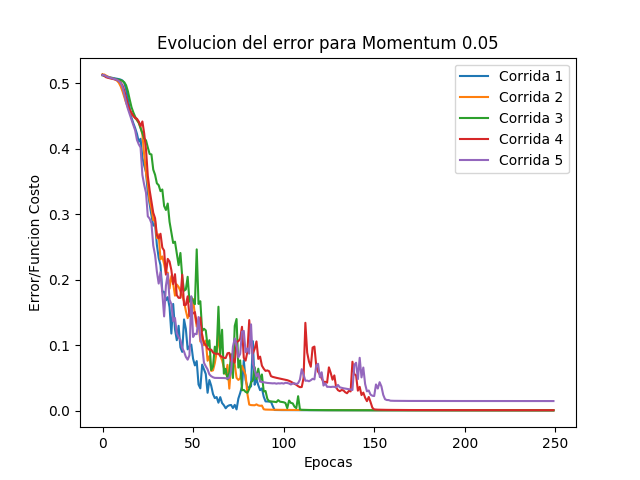
\includegraphics[width=1\linewidth]{graficos/momentum_0_05.png}
  \caption{Evolución del error de entrenamiento para momentum 0.05}
  \label{fig:sub2}
\end{subfigure}
\end{figure}

\begin{figure}[!htbp]
\centering
\begin{subfigure}{.5\textwidth}
  \centering
  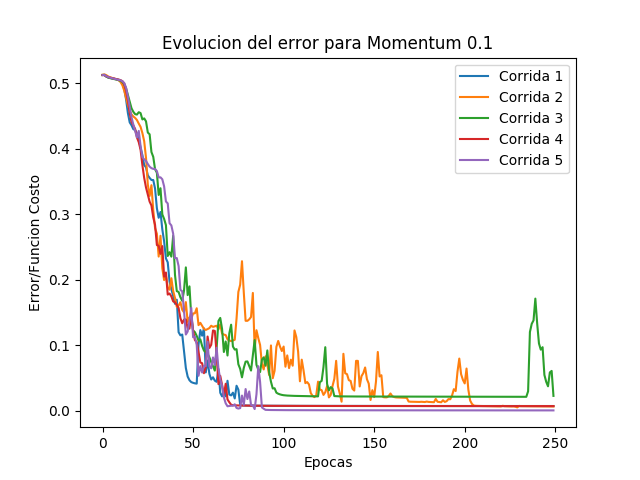
\includegraphics[width=1\linewidth]{graficos/momentum_0_1.png}
  \caption{Evolución del error de entrenamiento para momentum 0.1}
  \label{fig:sub1}
\end{subfigure}%
\begin{subfigure}{.5\textwidth}
  \centering
  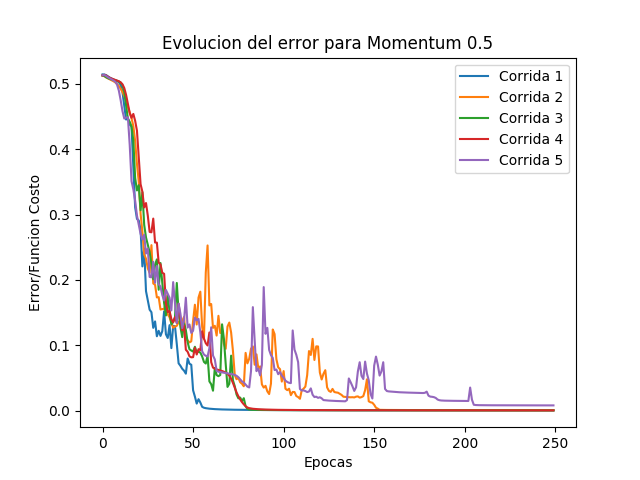
\includegraphics[width=1\linewidth]{graficos/momentum_0_5.png}
  \caption{Evolución del error de entrenamiento para momentum 0.5}
  \label{fig:sub2}
\end{subfigure}
\end{figure}

\begin{figure}[!htbp]
\centering
\begin{subfigure}{.5\textwidth}
  \centering
  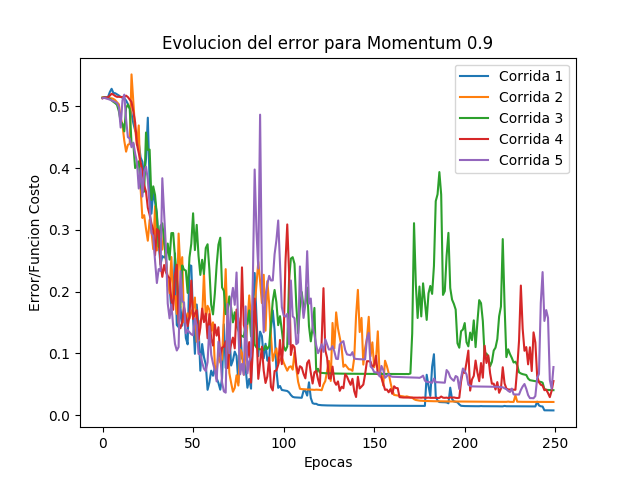
\includegraphics[width=1\linewidth]{graficos/momentum_0_9.png}
  \caption{Evolución del error de entrenamiento para momentum 0.9}
  \label{fig:sub1}
\end{subfigure}%
\begin{subfigure}{.5\textwidth}
  \centering
  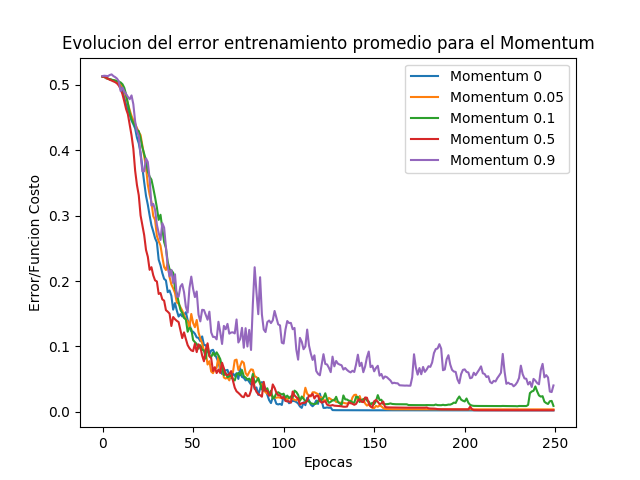
\includegraphics[width=1\linewidth]{graficos/momentum_promedios_entrenamiento.png}
  \caption{Evolución del error de entrenamiento promedio para todos los valores de momentum}
  \label{fig:sub2}
\end{subfigure}
\end{figure}

A partir de los resultados podemos intuir que manteniendo el learning rate elegido, no usar momentum o usar momentum $0.05$ o $0.5$ da los mejores resultados. Claramente
usar $0.9$ es casi como al nuevo peso de cada eje sumarle el peso anterior, por eso la oscilación tan pronunciada. Sin embargo, y para llegar a una conclusión del mejor 
valor de momentum, analizemos los resultados de la evolución del error para nuestro conjunto de validación:

\begin{figure}[!htbp]
  \begin{center}
  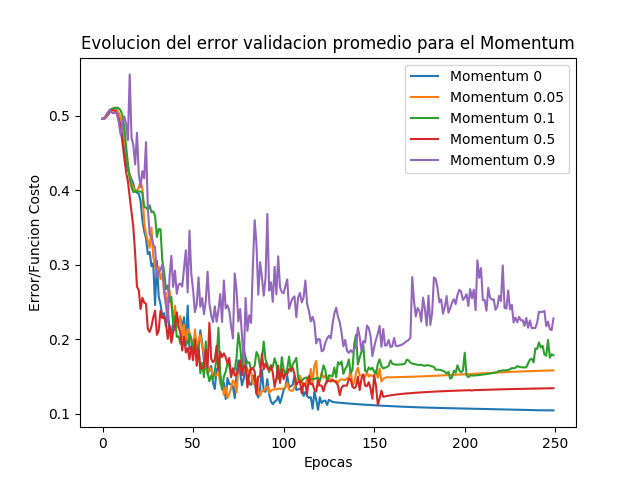
\includegraphics[scale=0.80]{graficos/momentum_promedios_validacion.png}
  \caption{Evolución del error de validación promedio para todos los valores de momentum}
  \end{center}
\end{figure}

Teniendo en cuenta ahora también nuestro error de validación final para todas las corridas y valores de momentum, podemos concluir entonces que manteniendo nuestro learning
rate fijo en $0.05$, lo mejor es no usar momentum.

\subsubsection{Performance de la red, con entrenamiento sin y con parámetros adaptativos.}

\subsubsection{Performance de la red, con entrenamiento estocástico, batch y mini-batch.}

\subsubsection{Performance de la red, variando simultáneamente el factor de aprendizaje $\mu$, y el parámetro $\alpha$ del momentum.}

\subsubsection{Performance de la red, con distintas técnicas de inicialización de los pesos de la red.}

\subsubsection{Performance de la red, sin y con preprocesamiento de los patrones.}

\subsubsection{Performance de la red, sin y con early-stopping.}

\subsubsection{Performance de la red, variando las funciones de activación y/o sus parámetros.}


\subsection{Descripción, justificación y performance, de la solución óptima propuesta.}


\subsection{Conclusiones.}